\documentclass[11pt,letterpaper]{scrartcl}

\usepackage{amsmath,amssymb,mathtools}
\usepackage{bm}
\usepackage[margin=0.82in]{geometry}
\usepackage{microtype}
\usepackage{booktabs}
\usepackage{array}
\usepackage{graphicx}
\usepackage{tikz}
\usepackage{scrlayer-scrpage}
\usepackage[hidelinks]{hyperref}

% Notation follows Chapter 5 of the book.
\newcommand{\dd}{\,\mathrm{d}}
\newcommand{\bU}{\bm{U}}
\newcommand{\bF}{\bm{F}}
\newcommand{\bK}{\bm{K}}

\definecolor{femblue}{HTML}{285F8F}
\graphicspath{{handouts/linear_finite_element_assembly/figures/}{figures/}}

\setlength{\parindent}{0pt}
\setlength{\parskip}{0.42em}
\setlength{\jot}{5pt}
\allowdisplaybreaks[1]
\emergencystretch=2em

\clearpairofpagestyles
\ihead{Advanced FEM}
\ohead{Linear finite element assembly}
\cfoot{\pagemark}
\pagestyle{scrheadings}

\begin{document}

\begin{center}
  {\Large\bfseries Local and Global Quantities for One-Dimensional Linear Elements}\\[4pt]
  {\large ME/BME 736 -- Advanced Finite Element Methods}\\[2pt]
  {\normalsize Prashant K. Jha}
\end{center}

\hrule
\vspace{0.7em}

This handout uses one three-element mesh to explain the distinction between
local and global quantities and how element load vectors and stiffness
matrices are assembled. The notation is the same as in Chapter~5.

\section{One mesh with local and global node numbers}

Let
\[
0=x_1<x_2<x_3<x_4=L
\]
be the global nodes of a mesh containing three elements:
\[
\mathcal K_1=(x_1,x_2),\qquad
\mathcal K_2=(x_2,x_3),\qquad
\mathcal K_3=(x_3,x_4).
\]

\begin{center}
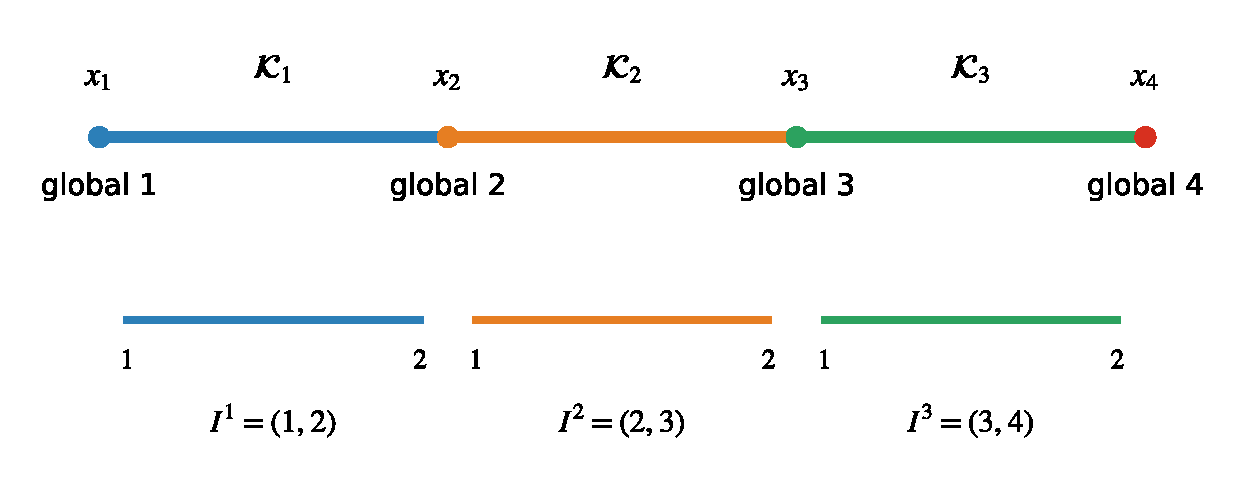
\includegraphics[width=0.80\textwidth]{local_global_numbering.pdf}
\end{center}

The global node numbers identify nodes in the complete mesh. The local node
numbers restart at $1$ and $2$ on every element. Thus the same physical node
$x_2$ is local node $2$ of element $1$ and local node $1$ of element $2$.

\subsection{The three maps used in assembly}

The local-to-global map $I^e$ tells us the global number of a local node:
\[
\begin{array}{c|cc}
e&I^e(1)&I^e(2)\\ \hline
1&1&2\\
2&2&3\\
3&3&4
\end{array}
\qquad\Longrightarrow\qquad
I^e(1)=e,\quad I^e(2)=e+1.
\]

The inverse map $J^e$ is used only on element $e$. If global node $i$ belongs
to element $e$, then $J^e(i)$ gives its local number on that element. For
example,
\[
J^1(2)=2,
\qquad
J^2(2)=1.
\]
The superscript is necessary because global node $2$ has a different local
number in the two elements that meet there.

Finally, let $\mathcal E(i)$ denote the elements attached to global node $i$.
For this mesh,
\begin{equation}
\mathcal E(1)=\{1\},\qquad
\mathcal E(2)=\{1,2\},\qquad
\mathcal E(3)=\{2,3\},\qquad
\mathcal E(4)=\{3\}.
\label{eq:incident-elements}
\end{equation}
Thus
\[
\begin{array}{rcl}
I^e(a)&:&\text{local node $a$ goes to which global node?}\\
J^e(i)&:&\text{global node $i$ has which local number on element $e$?}\\
\mathcal E(i)&:&\text{which elements meet at global node $i$?}
\end{array}
\]

\section{A global finite element function on one element}

Let $\{\phi_i\}_{i=1}^4$ be the global nodal basis. The basis function $\phi_i$
has value one at global node $i$ and zero at every other global node:
\begin{equation}
\phi_i(x_j)=\delta_{ij}.
\label{eq:global-nodal-property}
\end{equation}
The support of $\phi_i$ is defined by
\begin{equation}
\operatorname{supp}\phi_i
=\overline{\{x\in[0,L]:\phi_i(x)\ne0\}}.
\label{eq:support-definition}
\end{equation}
For the linear nodal basis, this support is the union of the closed elements
attached to node $i$:
\begin{equation}
\operatorname{supp}\phi_i
=\bigcup_{e\in\mathcal E(i)}\overline{\mathcal K}_e.
\label{eq:global-basis-support}
\end{equation}
Thus an interior basis function is supported on the two elements that meet at
its node, while an endpoint basis function is supported on one element.

\begin{center}
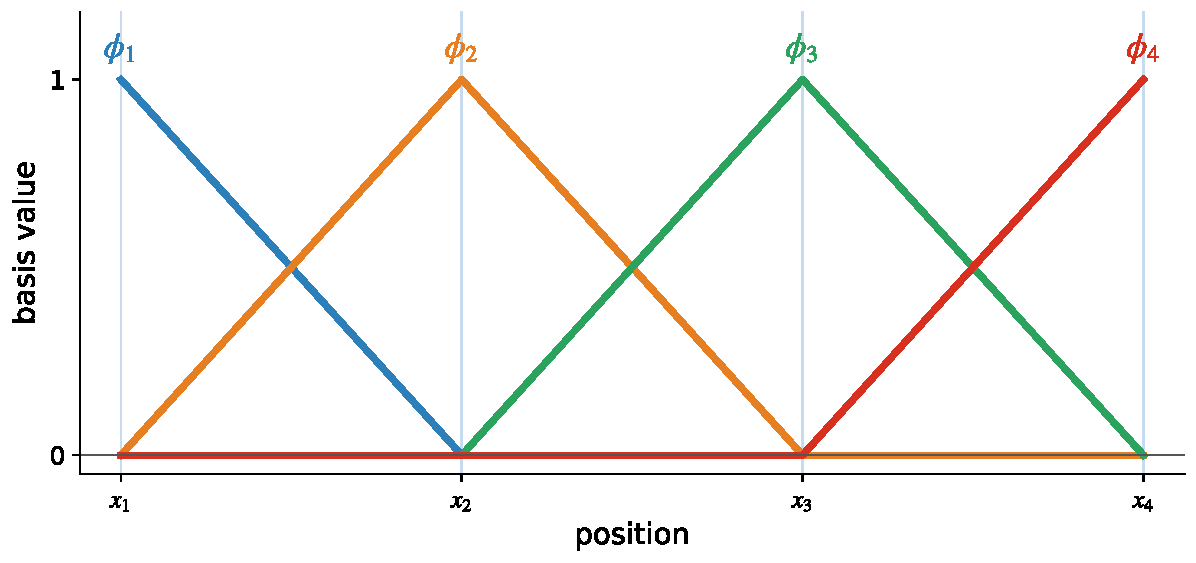
\includegraphics[width=0.74\textwidth]{global_linear_basis.pdf}
\end{center}

A finite element function is written globally as
\begin{equation}
u_h(x)=\sum_{i=1}^{4}U_i\phi_i(x).
\label{eq:global-function}
\end{equation}
The global degree of freedom $U_i$ is the nodal value $u_h(x_i)$.

On element $\mathcal K_e$, only the basis functions associated with its two
nodes are nonzero. Number the two local nodes from left to right and define
their coordinates by
\begin{equation}
x_1^e=x_e,
\qquad
x_2^e=x_{e+1}.
\label{eq:local-node-coordinates}
\end{equation}
The corresponding local degrees of freedom are
\begin{equation}
U_1^e=u_h(x_1^e),
\qquad
U_2^e=u_h(x_2^e).
\label{eq:local-dofs}
\end{equation}
Let $\phi_1^e$ and $\phi_2^e$ be the local basis functions:
\begin{equation}
\phi_1^e(x)=\frac{x_{e+1}-x}{h_e},
\qquad
\phi_2^e(x)=\frac{x-x_e}{h_e},
\qquad h_e=x_{e+1}-x_e.
\label{eq:local-basis}
\end{equation}
They satisfy $\phi_a^e(x_b^e)=\delta_{ab}$. Consequently, the restriction of
$u_h$ to element $e$ is first written entirely in local quantities as
\begin{equation}
\boxed{
u_h|_{\mathcal K_e}=U_1^e\phi_1^e+U_2^e\phi_2^e.
}
\label{eq:local-function-restriction}
\end{equation}

The local-to-global map identifies the same nodes in global notation:
\begin{equation}
U_a^e=U_{I^e(a)},
\qquad
\phi_a^e=\phi_{I^e(a)}|_{\mathcal K_e},
\qquad a=1,2.
\label{eq:local-global-dofs-and-basis}
\end{equation}
Substituting these relations into Equation
\eqref{eq:local-function-restriction} gives
\begin{equation}
\boxed{
u_h|_{\mathcal K_e}
=\sum_{a=1}^2U_{I^e(a)}\phi_a^e
=U_{I^e(1)}\phi_1^e+U_{I^e(2)}\phi_2^e.
}
\label{eq:function-restriction}
\end{equation}
For the consecutive numbering used here, $I^e(1)=e$ and $I^e(2)=e+1$, so the
two coefficients in Equation~\eqref{eq:function-restriction} are $U_e$ and
$U_{e+1}$.

\begin{center}
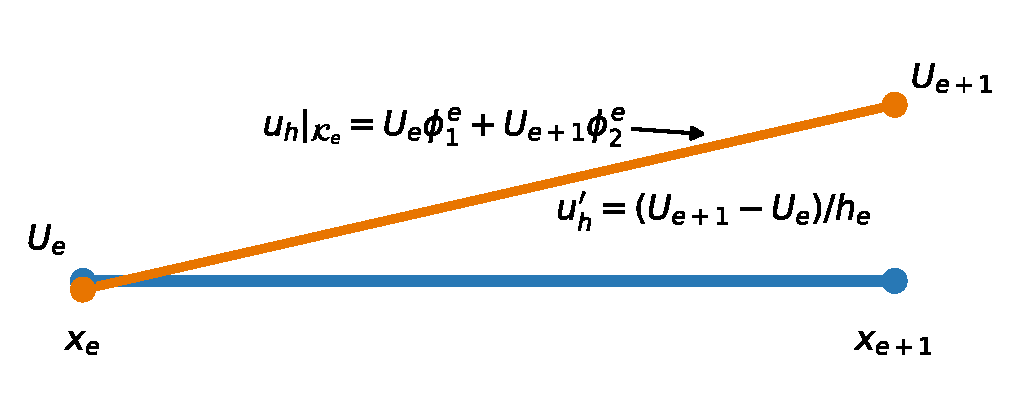
\includegraphics[width=0.70\textwidth]{linear_element_interpolation.pdf}
\end{center}

For example, $I^2=(2,3)$, and therefore
\begin{equation}
u_h|_{\mathcal K_2}=U_2\phi_1^2+U_3\phi_2^2,
\qquad
\bU^2=\begin{bmatrix}U_2\\U_3\end{bmatrix}.
\label{eq:element-two-function}
\end{equation}
For all three elements, the local coefficient vectors are
\[
\bU^1=\begin{bmatrix}U_1\\U_2\end{bmatrix},\qquad
\bU^2=\begin{bmatrix}U_2\\U_3\end{bmatrix},\qquad
\bU^3=\begin{bmatrix}U_3\\U_4\end{bmatrix}.
\]

\section{Assembly of the load vector}

For a distributed load $f$, the global load entry is
\begin{equation}
F_i=\int_0^L f\phi_i\,\dd x.
\label{eq:global-load-entry}
\end{equation}
Splitting the integral over all three elements first gives
\begin{equation}
F_i
=\sum_{e=1}^{3}
\int_{\mathcal K_e}f\phi_i\,\dd x.
\label{eq:global-load-full-sum}
\end{equation}
If element $e$ does not belong to $\mathcal E(i)$, then
$\phi_i|_{\mathcal K_e}=0$, and its integral in Equation
\eqref{eq:global-load-full-sum} is zero. The full sum therefore reduces to
\begin{equation}
F_i
=\sum_{e\in\mathcal E(i)}
\int_{\mathcal K_e}f\phi_i\,\dd x.
\label{eq:global-load-incident-sum}
\end{equation}
Define the two local load entries on element $e$ by
\begin{equation}
F_a^e=\int_{\mathcal K_e}f\phi_a^e\,\dd x,
\qquad a=1,2.
\label{eq:local-load-entry}
\end{equation}
Because $\phi_i|_{\mathcal K_e}=\phi_{J^e(i)}^e$, Equation
\eqref{eq:global-load-incident-sum} becomes
\begin{equation}
\boxed{
F_i=\sum_{e\in\mathcal E(i)}F_{J^e(i)}^e.
}
\label{eq:load-entry-assembly}
\end{equation}

For the three-element mesh,
\begin{align*}
F_1&=F_1^1,&
F_2&=F_2^1+F_1^2,&
F_3&=F_2^2+F_1^3,&
F_4&=F_2^3.
\end{align*}
Thus the global load vector is the sum of the three element vectors placed in
their global positions:
\begin{equation}
\boxed{
\bF
=
\begin{bmatrix}F_1^1\\F_2^1\\0\\0\end{bmatrix}
+
\begin{bmatrix}0\\F_1^2\\F_2^2\\0\end{bmatrix}
+
\begin{bmatrix}0\\0\\F_1^3\\F_2^3\end{bmatrix}
=
\begin{bmatrix}
F_1^1\\
F_2^1+F_1^2\\
F_2^2+F_1^3\\
F_2^3
\end{bmatrix}.
}
\label{eq:global-load-vector}
\end{equation}
At a shared node, the contributions from the neighboring elements are added.

\section{Assembly of the stiffness matrix}

The global stiffness entry for the axial bar is
\begin{equation}
K_{ij}=\int_0^L AE\,\phi_j'\phi_i'\,\dd x.
\label{eq:global-stiffness-entry}
\end{equation}
Define the local stiffness entries on element $e$ by
\begin{equation}
K_{ab}^e
=\int_{\mathcal K_e}AE\,(\phi_b^e)'(\phi_a^e)'\,\dd x,
\qquad a,b=1,2.
\label{eq:local-stiffness-entry}
\end{equation}
An element contributes to $K_{ij}$ only when it contains both global nodes
$i$ and $j$. Hence
\begin{equation}
\boxed{
K_{ij}
=\sum_{e\in\mathcal E(i)\cap\mathcal E(j)}
K_{J^e(i),J^e(j)}^e.
}
\label{eq:stiffness-entry-assembly}
\end{equation}
For example,
\[
K_{22}=K_{22}^1+K_{11}^2,
\qquad
K_{23}=K_{12}^2,
\qquad
K_{14}=0.
\]

Let
\[
\bK^e=
\begin{bmatrix}K_{11}^e&K_{12}^e\\K_{21}^e&K_{22}^e\end{bmatrix}.
\]
Placing each $2\times2$ element matrix into the rows and columns specified by
$I^e$ gives
\begin{align}
\bK
&=
\begin{bmatrix}
K_{11}^1&K_{12}^1&0&0\\
K_{21}^1&K_{22}^1&0&0\\
0&0&0&0\\
0&0&0&0
\end{bmatrix}
+
\begin{bmatrix}
0&0&0&0\\
0&K_{11}^2&K_{12}^2&0\\
0&K_{21}^2&K_{22}^2&0\\
0&0&0&0
\end{bmatrix}
\nonumber\\
&\quad+
\begin{bmatrix}
0&0&0&0\\
0&0&0&0\\
0&0&K_{11}^3&K_{12}^3\\
0&0&K_{21}^3&K_{22}^3
\end{bmatrix}
\nonumber\\[2pt]
&=
\begin{bmatrix}
K_{11}^1&K_{12}^1&0&0\\
K_{21}^1&K_{22}^1+K_{11}^2&K_{12}^2&0\\
0&K_{21}^2&K_{22}^2+K_{11}^3&K_{12}^3\\
0&0&K_{21}^3&K_{22}^3
\end{bmatrix}.
\label{eq:global-stiffness-matrix}
\end{align}

For a linear bar element with constant $AE$,
\begin{equation}
\bK^e
=\frac{(AE)_e}{h_e}
\begin{bmatrix}1&-1\\-1&1\end{bmatrix}.
\label{eq:bar-element-matrix}
\end{equation}
If $k_e=(AE)_e/h_e$, the assembled matrix is
\begin{equation}
\bK=
\begin{bmatrix}
k_1&-k_1&0&0\\
-k_1&k_1+k_2&-k_2&0\\
0&-k_2&k_2+k_3&-k_3\\
0&0&-k_3&k_3
\end{bmatrix}.
\label{eq:assembled-bar-matrix}
\end{equation}

\section{The assembly rule}

For every element $e$, compute its two local load entries and its four local
stiffness entries. Then use $I^e$ to add them to the global vector and matrix:
\begin{equation}
\boxed{
F_{I^e(a)}\mathrel{+}=F_a^e,
\qquad
K_{I^e(a),I^e(b)}\mathrel{+}=K_{ab}^e.
}
\label{eq:assembly-rule}
\end{equation}
The corresponding algorithm is
{\small
\begin{verbatim}
initialize F = 0 and K = 0
for each element e = 1,...,N:
    compute F^e and K^e
    for a = 1,2:
        i = I^e(a)
        F_i += F_a^e
        for b = 1,2:
            j = I^e(b)
            K_ij += K_ab^e
\end{verbatim}
}

In Python, subtract one from every mathematical node and element number when
using an array index. The mathematical derivation itself remains one-based.

\end{document}
